\subsection{Giả định, ràng buộc và rủi ro}
Hệ thống hướng tới quán nhỏ/vừa, barista kiêm xử lý thanh toán. Quản lý là stakeholder chốt chính sách; các vai trò truy cập được tổ chức thành CUSTOMER và BARISTA. Tiền VND lưu bằng số nguyên; frontend không truy cập PostgreSQL hoặc tự quyết định khoản thu. Khách chọn món vào giỏ chưa giữ kho; chỉ tạo Order hợp lệ mới giữ nguyên liệu.

Các rủi ro chính là tranh chấp phần cuối, gửi lặp đơn/callback, tiền về muộn, thu dư, đơn bỏ thanh toán giữ hàng, giá thay đổi trong lúc chờ đổi và hồ sơ bị hai nhân viên xử lý cùng lúc. Khóa dòng/transaction, unique key, snapshot và version giải quyết các rủi ro khác nhau. Timeout không chứng minh giao dịch thất bại hoặc ngân hàng đã hoàn tiền.

Tác vụ nền xử lý đơn hết thời gian giữ món dựa trên deadline lưu ở database. VNPay được sử dụng trong môi trường Sandbox; khoản thu không áp dụng được quầy xử lý theo hồ sơ và chứng từ. Nhu cầu giao hàng được ghi nhận ở mức nghiệp vụ; phạm vi giao diện tập trung khách và quầy. 

\subsection{Sơ đồ use-case}
Hai sơ đồ tóm tắt phạm vi chức năng và tương tác trong luồng đặt, thanh toán đơn.
\begin{figure}[htbp]\centering
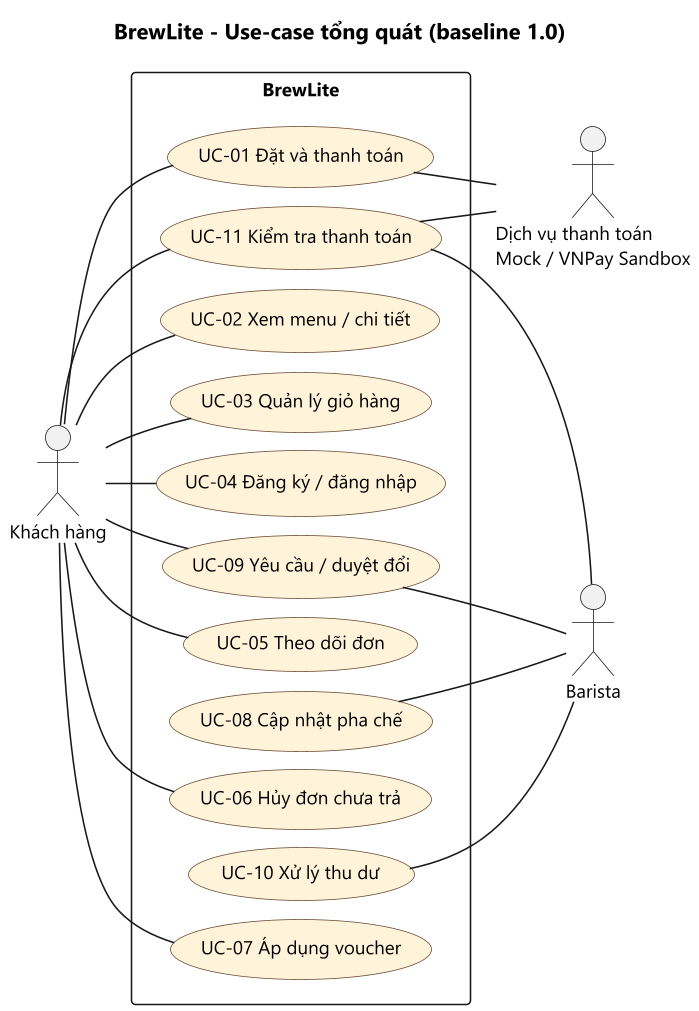
\includegraphics[width=.95\linewidth,height=.68\textheight,keepaspectratio]{../docs/diagrams/usecase-system.png}
\caption{Use-case tổng quát, có nguồn PlantUML và bản SVG trong docs/diagrams}
\end{figure}
\begin{figure}[htbp]\centering
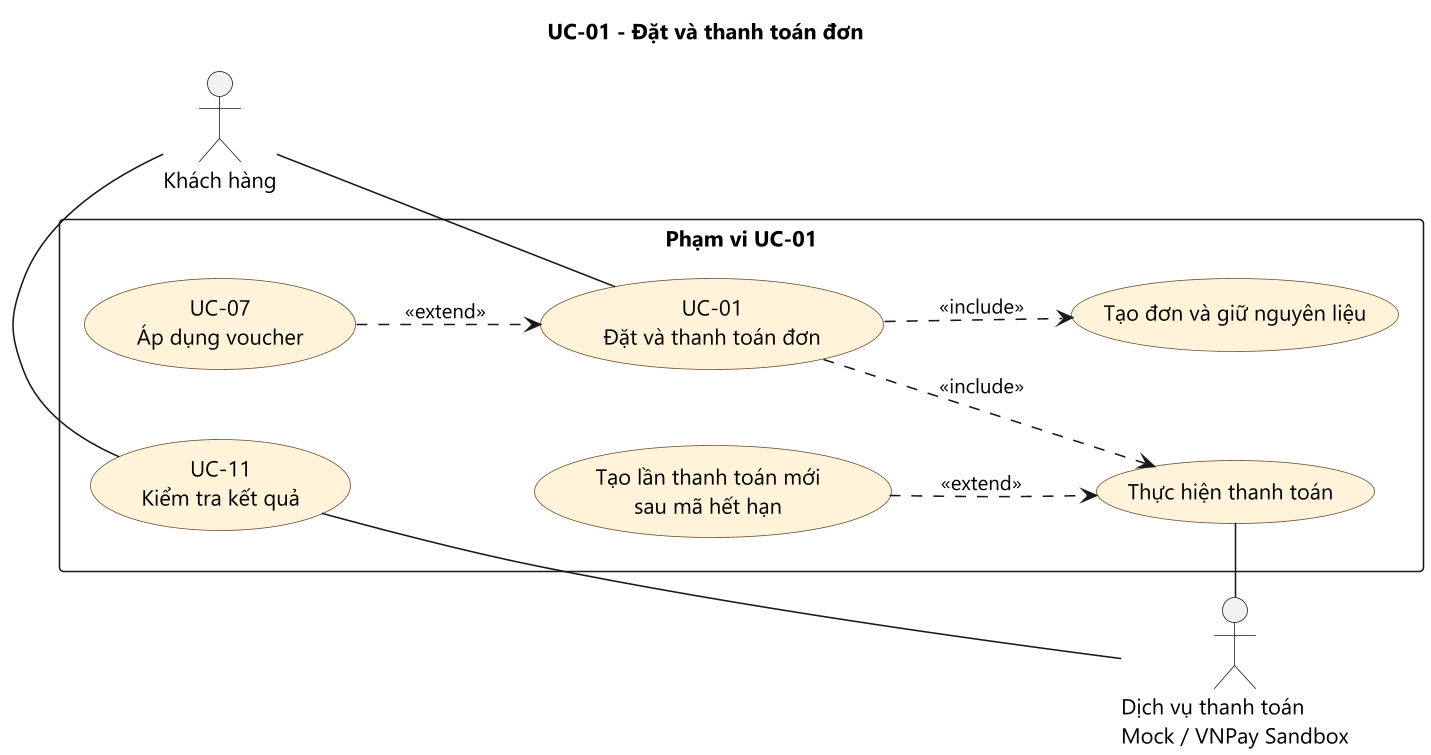
\includegraphics[width=\linewidth,height=.48\textheight,keepaspectratio]{../docs/diagrams/usecase-checkout.png}
\caption{Phạm vi UC-01: đặt và thanh toán đơn}
\end{figure}
